\scanpage{12}
\mspage{30}
\margin{\unsure{1}}
\deleted{
\deleted{on a nécessairement} puisque ses composantes connexes sont ouvertes ($S$
étant localement noethérien). Mais alors on a nécessairement $Z=J_S$,
où $J$ est une partie de $I$, et on a \deleted{\unsure{donc}} donc $U=\varnothing$ ou $U=S$, suivant que $J$
est infini ou fini, ce qui donne la conclusion voulue.

\uline{Corollaire} 5.14. Soi\deleted{t}\inserted{ent} $S$ un préschéma localement noethérien et \uline{normal},
$\deleted{\unsure{R}}\inserted{P}$ un $S$-préschéma \deleted{localement} constant tordu quasi-isotrivial. Alors les
composantes connexes de $\deleted{\unsure{R}}\inserted{P}$ sont finies sur $S$.

Comme $\deleted{\unsure{R}}\inserted{P}$ est étale sur $S$, on sait que $\deleted{\unsure{R}}\inserted{P}$ est normal (SGA I 9.5.)
donc ses composantes \deleted{irréductibles} connexes sont ses composantes
irréductibles. On peut évidemment supposer $S$ connexe donc irréductible,
soit $s$ son point générique. Comme $R$ est plat sur $S$, ses points maximaux,
i.e. les points génériques $x_i$ des composantes irréductibles $R_i$ de $R$,
sont les points maximaux de $R_s$, et la fibre \deleted{\unsure{de R}} générique $R_{i\,s}$ de $R_i$
est la composante irréductible de $R_s$, adhérence de $x_i$ dans $R_s$. Or
$R_s$ étant étale sur $k(s)$, est somme disjointe de spectres \unsure{dr'extensions|d'extensions}
finies séparables de $k(s)$, donc \deleted{les} pour tout $i$, $R_{i\,s}$ est fini (en
fait, réduit à un seul point). Donc 5.13. s'applique et montre que
les $R_i$ sont finis sur $S$.

\uline{Remarque} 5.15. Le raisonnement s'applique, plus généralement, si on
suppose seulement $S$ géométriquement unibranche au lieu de normal, i.e.
que le morphisme \unsure{Canonique|canonique} $\widetilde S\longrightarrow S$, où $\widetilde S$ est le normalisé de $S_{\text{réd}}$,
est radiciel. Donc le théorème 5.16. ci-dessous est valable également
sous cette condition plus générale.

\uline{Théorème} 5.16. Soit $S$ un préschéma localement noethérien normal. Alors
tout groupe de type multiplicatif \deleted{\unsure{de type fini}} \inserted{et de type fini} sur $S$ \deleted{\unsure{local et en parti}}
est \uline{isotrivial}.
\inserted{\uline{On peut} supposer en effet \inserted{\figure{\begin{tikzpicture}[baseline=(n.base)]\node[draw,ellipse,inner sep=1pt] (n) {$S$ connexe, donc};\end{tikzpicture}}} $H$ de type constant $M$.}
Il suffit d'appliquer 5.13 . avec $P=\underline{\operatorname{Isom}}_{S\text{-gr}}(H,G)$, où $G=D_S(M)$,
}
\inserted{en raisonnant comme dans \unsure{5.10|5.14}. (ii)$\Longrightarrow$(i); \uline{on peut aussi} \unsure{appli-}\\
ou \deleted{\unsure{encore}} \unsure{5.11}. \deleted{\illegible{3}}, en utilisant \unsure{5.14} pour $R=D_S(\unsure{\check H|\check M})$.}
\margin{\unsure{5.11}.}
\margin{\figure{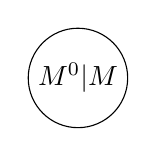
\begin{tikzpicture}[baseline=(n.base)]\node[draw,circle,inner sep=2pt] (n) {$\unsure{M^0|M}$};\end{tikzpicture}}}
\mspage{\unsure{11|M}}

